\documentclass[portuguese,10pt,xcolor=table]{beamer}
\setbeameroption{show notes}

\usepackage[brazil]{babel}
\usepackage[utf8]{inputenc}
\usepackage{times}
\usepackage{varwidth}
\usepackage{listings}
\usepackage{tikz}
\usepackage[tikz]{bclogo}
\usetikzlibrary{arrows,shapes}

\definecolor{deepgreen}{rgb}{0,0.5,0}
\lstset{
	language=C,
	basicstyle=\footnotesize\ttfamily,
	%basicstyle=\scriptsize\ttfamily,
	keywordstyle=\footnotesize\bfseries\sffamily,
	%keywordstyle=\scriptsize\bfseries\sffamily,
	showstringspaces=false,
	numbers=left,
	numberstyle=\footnotesize,
	stepnumber=1,
	numbersep=5pt,
	tabsize=4,
	%backgroundcolor=\color{blue!05},
	backgroundcolor=\color{gray!35},
	showspaces=false,
	showtabs=false,
	stringstyle=\ttfamily\color{red!80!brown},
	commentstyle=\ttfamily\color{blue!80},
	keywordstyle=\bfseries\color{deepgreen},
	escapeinside={\%*}{*)}
}
\renewcommand{\lstlistingname}{Código}

\usetikzlibrary{calc,decorations.pathmorphing,patterns}
\pgfdeclaredecoration{penciline}{initial}{
	\state{initial}[width=+\pgfdecoratedinputsegmentremainingdistance,
		auto corner on length=1mm,]{
			\pgfpathcurveto%
			{% From
				\pgfqpoint{\pgfdecoratedinputsegmentremainingdistance}
				{\pgfdecorationsegmentamplitude}
			}
			{%  Control 1
				\pgfmathrand
					\pgfpointadd{\pgfqpoint{\pgfdecoratedinputsegmentremainingdistance}{0pt}}
				{\pgfqpoint{-\pgfdecorationsegmentaspect
							   \pgfdecoratedinputsegmentremainingdistance}%
							   {\pgfmathresult\pgfdecorationsegmentamplitude}
				}
			}
			{%TO 
				\pgfpointadd{\pgfpointdecoratedinputsegmentlast}{\pgfpoint{1pt}{1pt}}
			}
		}
	\state{final}{}
}



\everymath{\displaystyle}
\tikzstyle{every picture}+=[remember picture,decoration=penciline]
\DeclareTextFontCommand{\textdf}{\bfseries\color{blue!80}}
%\tikzstyle{every node}+=[decorate]
%\tikzstyle{every path}+=[decorate]
%\tikzstyle{na} = [baseline=-.5ex]

\usepackage[T1]{fontenc}

\def\lecturename{IMD0012 - Introdução às técnicas de programação}

\title{\insertlecture}

\author{Prof. Fernando Figueira\\(adaptado do material do Prof. Rafael Beserra Gomes)}

\institute{UFRN}

\subject{Introdução a programação em C}

\lecture[]{Operadores}{}

%\subtitle{Introdução}

\date{}

\def\exe[#1]{\color{gray}#1\color{black}}
\def\exp[#1]{\color{gray}<\textit{#1}>\color{black}}
\def\espaco{\color{gray}\hspace{0.2cm}\color{black}}

\begin{document}

\usebackgroundtemplate{%
	
\includegraphics[width=\paperwidth,height=\paperheight]{background2}
}
\begin{frame}
  \maketitle
 \begin{center}
 \tiny
Material compilado em \today.\\
  Licença desta apresentação:\\
		
\includegraphics[height=1.0cm]{by-nc-nd.png}\\
http://creativecommons.org/licenses/
	\end{center}
\end{frame}

	\section{Expressões}
	\begin{frame}
	\begin{itemize}
		\item Combinação de \textdf{valores}, \textdf{variáveis}, \textdf{operadores} e \textdf{chamadas de funções}.
		\item São resolvidas durante a compilação ou durante a execução
	\end{itemize}

	\end{frame}


	\section{Tipos de operadores}
	\begin{frame}
		\textdf{Operadores} realizam uma funcionalidade específica com os \textdf{operandos}.
		\vspace{0.5cm}
	
		Categorias dos operadores desta disciplina:
		\begin{itemize}
			\item Operadores aritméticos
			\item Operadores de atribuição
			\item Operadores relacionais
			\item Operadores lógicos
		\end{itemize}
	\end{frame}

	\section{Op. aritméticos}
	\begin{frame}
		\textdf{Operadores aritméticos}
		\begin{itemize}
			\item +, -, *, /, \%
			\item todos esses são binários (dois operandos numéricos)
			\item Exemplo:
			\lstinputlisting{operadorAritmetico.c}
		\end{itemize}
	\end{frame}
	
	\section{Op. de atribuição}
	\begin{frame}
		\textdf{Operadores de atribuição}
		\begin{itemize}
			\item \exp[variável]\espaco=\espaco\exp[expressão]
			\item \exp[variável]\espaco+=\espaco\exp[expressão] (ou -=, *=, /=)
			\item Exemplo:
		        \lstinputlisting{operadorAtribuicao.c}
		\end{itemize}
	\end{frame}


\section{Op. lógicos}
   
    
    \begin{frame}
		\textdf{Operadores lógicos}: atua em \textdf{proposições}
    	\begin{itemize}
    		\item Uma proposição é uma sentença que pode ser avaliada como \textbf{verdadeira} ou \textbf{falsa}
    		\item Exemplos de proposições:
    			\begin{itemize}
    				\item p: O céu é azul
    				\item q: Natal é a capital da Paraíba
    			\end{itemize}
    			Exemplos de sentenças que não são proposições:
    			\begin{itemize}
    				\item r: Um evento fora da cidade
    			\end{itemize}
    	\end{itemize}
	\end{frame}

   \begin{frame}
	   \begin{itemize}
		   \item Em C declare as proposições como \textdf{int} (chamamos de variável lógica ou booleana)
		   \item \textdf{$= 0$} $\leftrightarrow$ \textdf{falso}
		   \item \textdf{$\ne 0$} $\leftrightarrow$ \textdf{verdadeiro}
		   \item Exemplo:
			   \lstinputlisting{logico1.c}
		   \item Por que variáveis lógicas?
			   \begin{itemize}
				   \item p: O usuário clicou no botão x
				   \item q: O CPF digitado não é um CPF válido
			   \end{itemize}
	   \end{itemize}

   \end{frame}


	\begin{frame}

		A \textdf{Tabela Verdade} exibe todos os resultados possíveis de um \textbf{operador lógico} em função dos valores dos operandos.
 
		\vspace{0.5cm}
		Vamos ver 3 operadores lógicos:
		\begin{itemize}
			\item negação
			\item disjunção (ou)
			\item conjunção (e)
		\end{itemize}
    \end{frame}
    
    \begin{frame}
		\textdf{Operador de negação (unitário): } !\\
    	\begin{tabular}{|l|l|}
    		\hline
    		\textbf{p} & \textbf{$!p$}\\
    		\hline
    		F& V\\
    		\hline
    		V& F\\
    		\hline
    	\end{tabular}\\\vspace{1cm}
    	Por exemplo:
    	\begin{itemize}
    		\item p: O céu é azul
    		\item seja $p = V$, !p = F
    	\end{itemize}
    \end{frame}
    
    \begin{frame}
		\textdf{Operador de disjunção (ou): } ||\\
    	\begin{tabular}{|l|l|l|}
    		\hline
    		\textbf{p} & \textbf{q} & \textbf{p || q}\\
    		\hline
    		F& F& F\\
    		\hline
    		V& F& V\\
    		\hline
    		F& V& V\\
    		\hline
    		V& V& V\\
    		\hline
    	\end{tabular}\\\vspace{1cm}
    	Por exemplo:
    	\begin{itemize}
    		\item p: O céu é azul
			\item q: Natal é a capital da Paraíba
    		\item seja $p = V$ e $q = F$, p || q = V
    	\end{itemize}
    \end{frame}
    
    \begin{frame}
		\textdf{Operador de conjunção (e): } \&\&\\
    	\begin{tabular}{|l|l|l|}
    		\hline
			\textbf{p} & \textbf{q} & \textbf{p \&\& q}\\
    		\hline
    		F& F& F\\
    		\hline
    		V& F& F\\
    		\hline
    		F& V& F\\
    		\hline
    		V& V& V\\
    		\hline
    	\end{tabular}\\\vspace{1cm}
    	Por exemplo:
    	\begin{itemize}
    		\item p: O céu é azul
			\item q: Natal é a capital da Paraíba
			\item seja $p = V$ e $q = F$, p \&\& q = F
    	\end{itemize}
    \end{frame}
    

\section{Operadores relacionais}
	\begin{frame}
	\textdf{Operadores relacionais}:
		
		\begin{itemize}
			\item resultam em valores lógicos (1 para verdadeiro ou 0 para falso)
			\item \textbf{==}: compara se os dois operandos são iguais
			\item \textbf{!=}: compara se os dois operandos são diferentes
			\item \textbf{>, <, >=, <=}: o mesmo significado matemático para $>, <, \ge , \le $
		\end{itemize}
		Observações:
		\begin{itemize}
			\item Os operadores => ou =< não existem
			\item Por que \textit{a > b > c} não realiza o seu respectivo significado matemático?
		\end{itemize}
	\end{frame}

\section{Precedência dos operadores}

	\begin{frame}
	\textdf{Precedência dos operadores vistos}:
		
    	\begin{tabular}{|l|l|}
    		\hline
			precedência & operadores \\\hline
			maior (avaliado primeiro) & ()\\
			& * / \%\\
			& + - \\
			& < <= >= > \\
			& == != \\
			& \&\& \\
			& || \\
			menor (avaliado por último) & = *= += -= \\\hline
    	\end{tabular}
	\end{frame}

\section{Chamadas de funções}

	\begin{frame}
		Escrever na tela o resultado de $2 \times 2^3$\\
			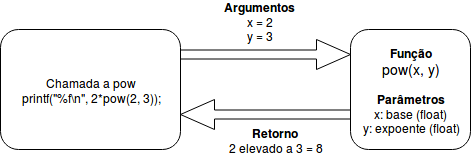
\includegraphics[height=3.0cm]{funcao1.png}\\
	\end{frame} 
	\begin{frame}
		Escrever na tela o resultado de $4^{3^2}$\\
			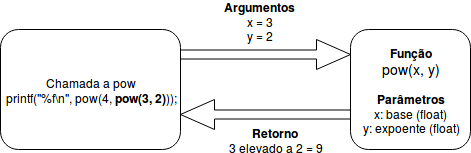
\includegraphics[height=3.0cm]{funcao2.png}\\
	\end{frame} 
	\begin{frame}
		Escrever na tela o resultado de $4^{3^2}$\\
			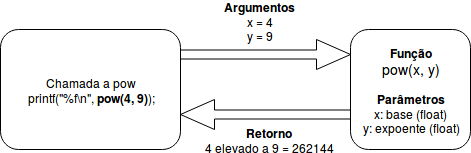
\includegraphics[height=3.0cm]{funcao3.png}\\
	\end{frame} 

	\begin{frame}
		Já utilizamos (\textit{chamamos}) várias funções:
		\begin{itemize}
			\item pow(x, y): \textdf{retorna} $x^y$
			\item sqrt(x): \textdf{retorna} a raiz quadrada de x
			\item printf(...): escreve na saída padrão e \textdf{retorna} a quantidade de caracteres escritos
			\item scanf(...): lê da entrada padrão e \textdf{retorna} a quantidade de elementos lidos com sucesso
			\item srand(x): altera a semente para a geração de números aleatórios
		\end{itemize}		
	\end{frame} 


	\begin{frame}
		Quais funções há em C e como utilizá-las?
				\begin{itemize}
					\item as funções estão organizadas em \textdf{bibliotecas}
					\item verifique a \textdf{assinatura} da função\\
						exemplo:        \textdf{double sqrt(double x);}

					\item consulte \textbf{man 3 nomefuncao} ou http://www.cplusplus.com/reference/clibrary/
				\end{itemize}
			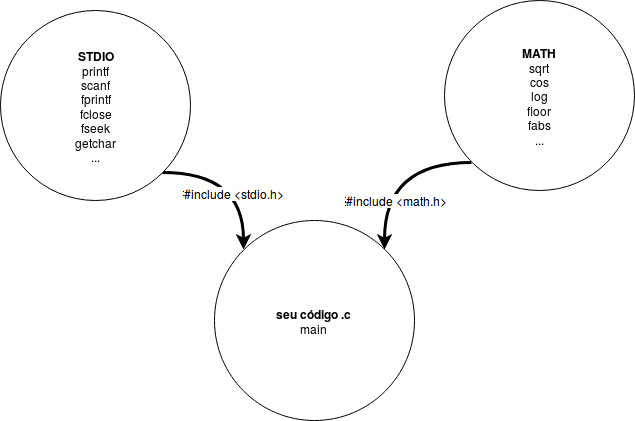
\includegraphics[height=4.5cm]{includes.png}
	\end{frame} 
	\begin{frame}
		Você pode incluir outras bibliotecas, exemplo:
				\begin{itemize}
					\item gtk+: para criar interfaces gráficas
					\item opengl: para gráficos 3D
					\item ...dentre tantas outras
				\end{itemize}
				Provavelmente exigirá a instalação da biblioteca (exemplo, para usar o gtk+ pode fazer no ubuntu: \textit{sudo apt-get install libgtk-3-dev})
			
			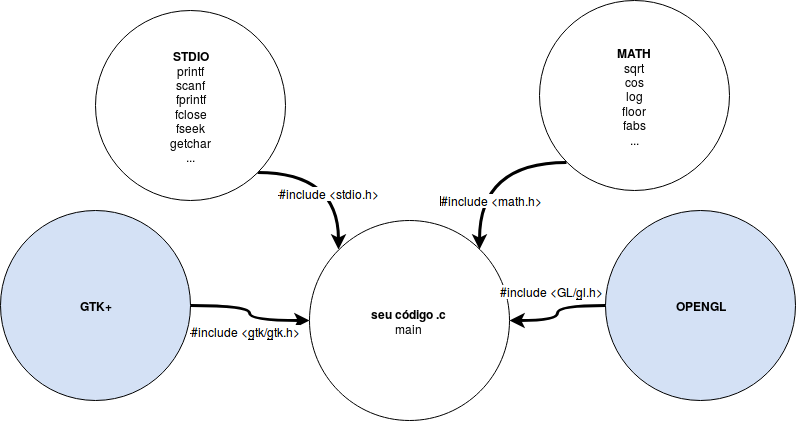
\includegraphics[height=4.5cm]{includes2.png}
	\end{frame}


\end{document}


